Client è composto da diverse classi che espongono le varie funzionalità sul modello. In particolare, la classe \texttt{Client} è una composizione di funzionalità fornite da:
\begin{itemize}
	\item \texttt{ExerciseClient}: fornisce le funzionalità di inserimento, risoluzione e ricerca degli esercizi;
	\item \texttt{ClassClient}: fornisce le funzionalità di inserimento e recupero delle informazioni delle classi e l'assegnazione degli esercizi;
	\item \texttt{UserClient}: fornisce le funzionalità di inserimento e verifica dell'identità degli utenti.
\end{itemize}

\begin{figure}[ht]
	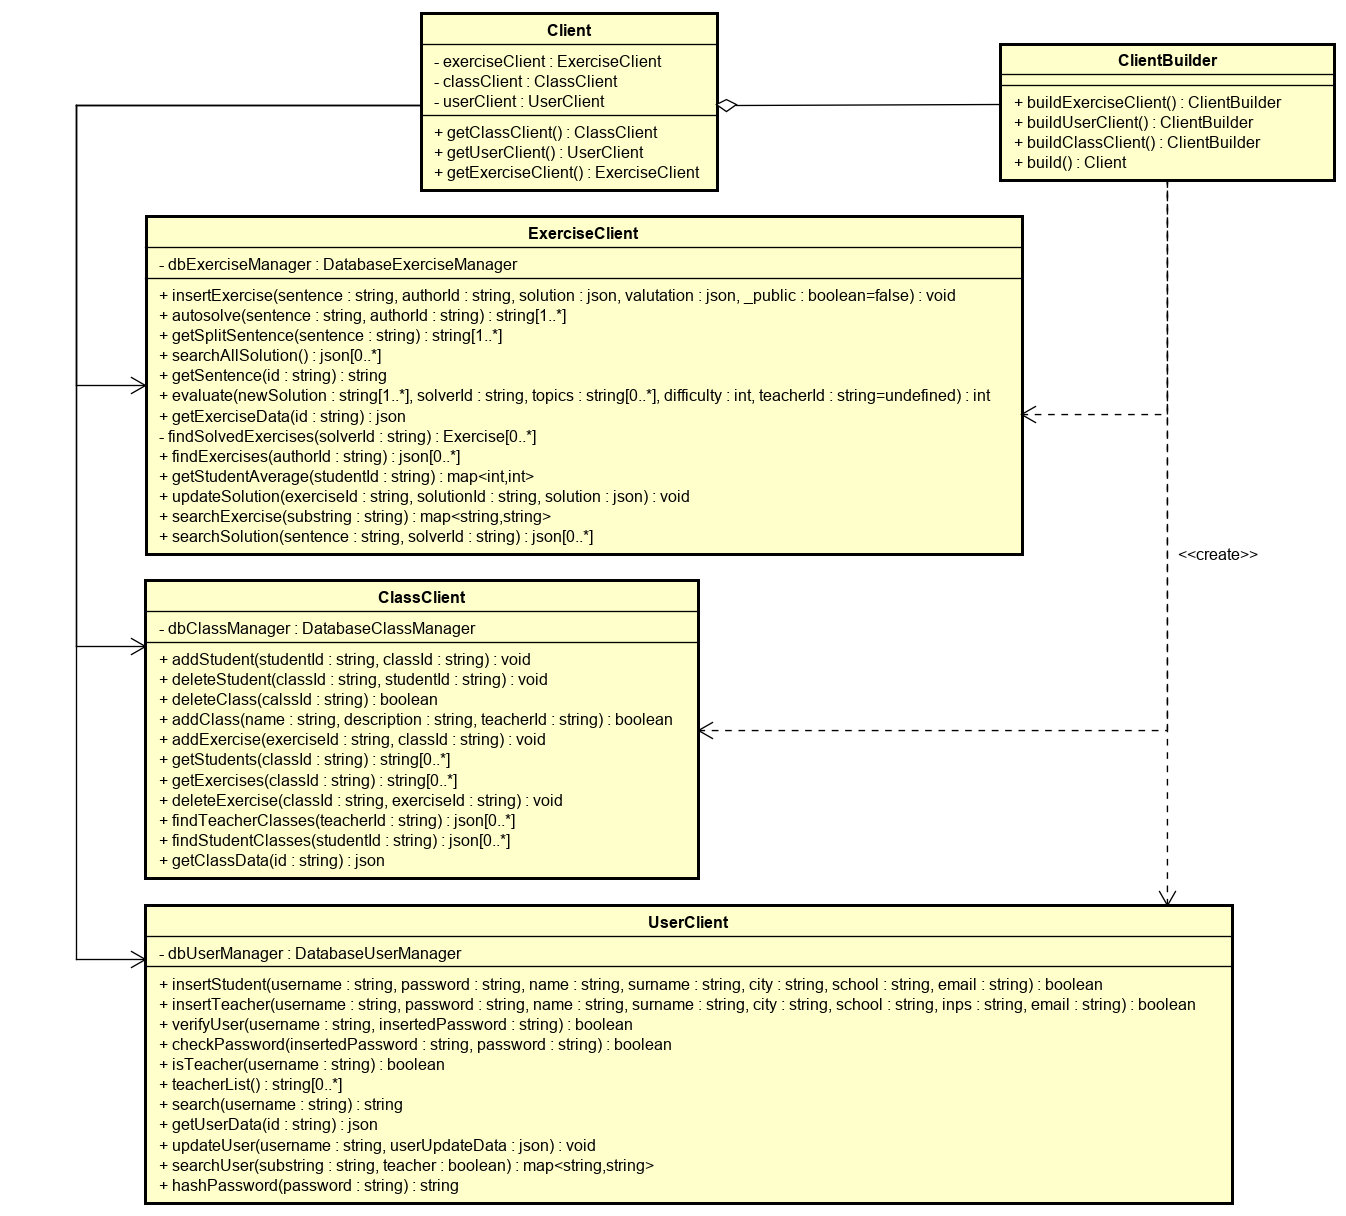
\includegraphics[scale=0.5]{images/Client.png}
	\caption{Diagramma delle classi del package Client}
\end{figure}